\section{Análisis estático automatizado de código}

	\subsection{Error nº1: Memory leak}

		\subsubsection{Origen/explicación del error detectado}
		
			\paragraph{}En las siguientes dos capturas de pantalla se muestra el código fuente de las funciones \textit{modifica} y \textit{elimina\_dato} de la clase plantilla \textit{lista\_sin} de nuestra aplicación.
			
			\begin{figure}[H]
				\centering
				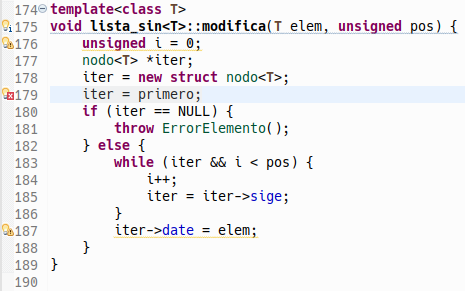
\includegraphics[scale=0.7]{img/captura42.png}
				\caption{Captura de pantalla de la función modifica}
				\label{captura42}
			\end{figure}
		
			\begin{figure}[H]
				\centering
				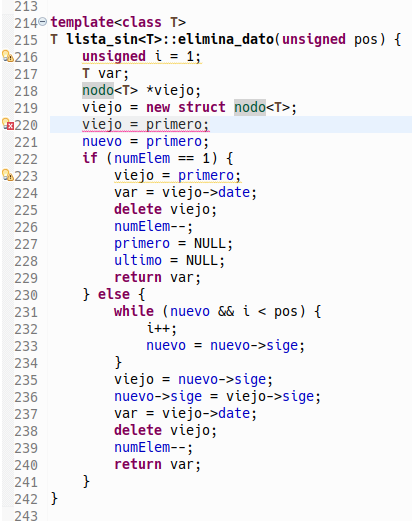
\includegraphics[scale=0.7]{img/captura45.png}
				\caption{Captura de pantalla de la función elimina\_dato}
				\label{captura45}
			\end{figure}
		
			\paragraph{}En la línea 179 cppchek nos indica que ha detectado un error de código, en concreto, se trata de un error de perdida de memoria para la variable \textit{iter}. Esto es debido a que en la línea 177 se declara la variable (la cual es un puntero a una estructura llamada \textit{nodo}, que hemos definido nosotros anteriormente en el mismo archivo), y en la línea 178 se inicializa con la palabra reservada \textit{new}. Al realizar esto anterior, hemos reservado memoria dinámica para la estructura y la hemos inicializado.
			
			\begin{figure}[H]
				\centering
				
\includegraphics[scale=0.38]{img/captura43.png}
				\caption{Detalle del mensaje de error de cppcheck}
				\label{captura43}
			\end{figure}
		
			\begin{figure}[H]
				\centering
				
\includegraphics[scale=0.38]{img/captura46.png}
				\caption{Detalle del mensaje de error de cppcheck}
				\label{captura46}
			\end{figure}
			
			\paragraph{}El error se origina cuando, en la línea 179, hacemos que la variable \textit{iter} (que es un puntero) apunte al atributo de la clase \textit{primero} sin liberar la memoria de la estructura con la que inicializamos anteriormente. Esto hace que la memoria que ocupa dicha estructura no se libere y que, por lo tanto, se produzca una pérdida de memoria. 
			
			\paragraph{}En el caso de la función \textit{elimina\_dao}, la explicación del origen del error es exactamente la misma pero aplicada a la variable \textit{viejo}.
		
		\subsubsection{Corrección realizada para solventar el error}
		
			\paragraph{}La manera de resolver esta incidencia es de lo más trivial. Tan solo deberemos realizar la declaración de la variable y, acto seguido, asignarle la dirección de memoria del atributo de la clase \textit{primero}. A continuación, dejamos una captura de pantalla del estado de las funciones tras la resolución de los errores:
			
			\begin{figure}[H]
				\centering
				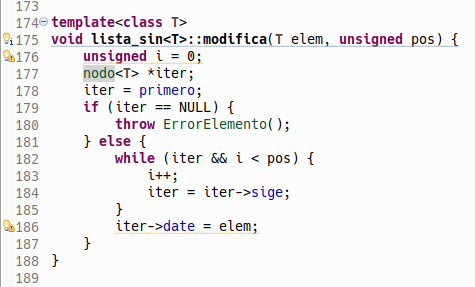
\includegraphics[scale=0.7]{img/captura44.png}
				\caption{Captura de pantalla de la función modifica tras la resolución del error}
				\label{captura44}
			\end{figure}
		
			\begin{figure}[H]
				\centering
				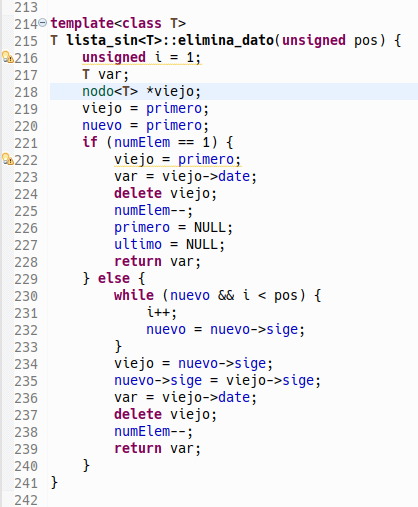
\includegraphics[scale=0.7]{img/captura47.png}
				\caption{Captura de pantalla de la función elimina\_dato}
				\label{captura47}
			\end{figure}
		
			\paragraph{nota:}Cabe destacar que también se podría haber resuelto este error realizando un $"delete$ $iter/viejo"$ antes de asignarle la dirección de memoria del atributo \textit{primero} pero en este caso hemos descartado esta opción ya que la estructura con la que se inicializa no se utiliza para nada y supondría la realización de operaciones adicionales innecesarias.
	
	\subsection{Error nº2: Mismatching allocation and deallocation}

		\subsubsection{Origen/explicación del error detectado}
		
			\paragraph{}A continuación presentamos una captura de pantalla de la función \textit{limpia} de la clase plantilla \textit{lista\_sin}.
		
			\begin{figure}[H]
				\centering
				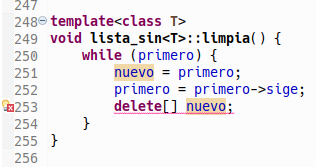
\includegraphics[scale=0.7]{img/captura48.png}
				\caption{Captura de pantalla de la función limpia}
				\label{captura48}
			\end{figure}
	
			\paragraph{}En esta función, en la línea 253, cppcheck nos indica que hay un error. Dicho error es originado dado que hacemos un $"delete[]"$, es decir, una liberación de memoria para un vector/array de punteros. En el caso de la variable \textit{nuevo}, podemos comprobar que se trata de un atributo de la clase \textit{lista\_sin} y que se trata de un puntero a una estructura llamada \textit{nodo}. Justo esto anterior es lo que genera el error, es decir, estamos intentando liberar la memoria asignada de un vector/array cuando la variable \textbf{no es ninguno de estos}.
		
			\begin{figure}[H]
				\centering
				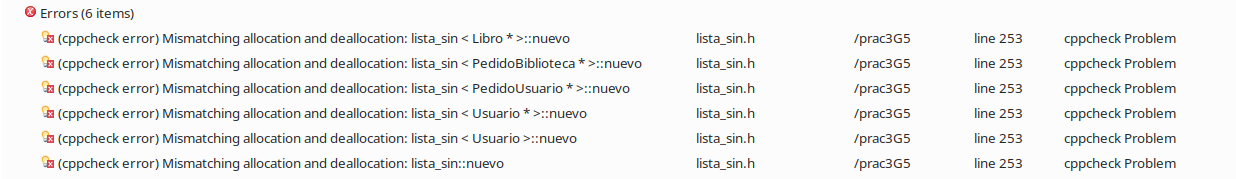
\includegraphics[scale=0.38]{img/captura49.png}
				\caption{Detalle del mensaje de error de cppcheck}
				\label{captura49}
			\end{figure}

		\subsubsection{Corrección realizada para solventar el error}
		
			\paragraph{}Para corregir este error lo único que deberemos realizar es sustituir la sentencia $"delete[]$ $nuevo"$ por la sentencia $"delete$ $nuevo"$. Una vez realizado esto el error habrá desaparecido, como se puede comprobar en la siguiente captura de pantalla:
		
			\begin{figure}[H]
				\centering
				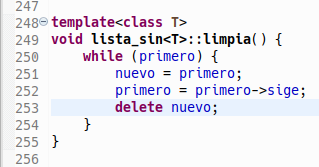
\includegraphics[scale=0.7]{img/captura50.png}
				\caption{Captura de pantalla de la función limpia tras la resolución del error}
				\label{captura50}
			\end{figure}
		
	\subsection{Error nº3: Class has a constructor with 1 argument that is not explicit}
	
		\subsubsection{Origen/explicación del error detectado}
	
			\paragraph{}En la siguiente captura de pantalla se observa el constructor parametrizado de la clase \textit{PedidoBiblioteca}.
			
			\begin{figure}[H]
				\centering
				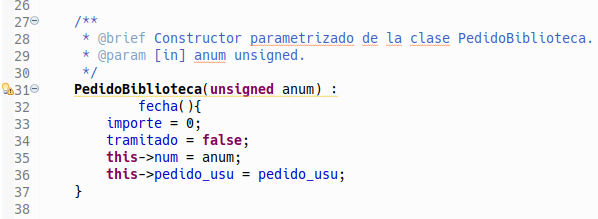
\includegraphics[scale=0.7]{img/captura51.png}
				\caption{Captura de pantalla del constructor parametrizado de la clase PedidoBiblioteca}
				\label{captura51}
			\end{figure}
		
			\paragraph{}Como se puede observar en la captura de pantalla, en este constructor se hace uso de una lista de inicializadores de miembro, la cual inicializa el valor de los atributos miembro antes de la ejecución del cuerpo del constructor.
			
			\paragraph{}En la lista observamos que se encuentra el atributo miembro \textit{fecha} inicializado con su constructor por defecto. Esto es debido a que entre paréntesis no hemos escrito ningún nombre de variable, ya que no se le pasa ningún parámetro del tipo fecha al constructor.
			
			\paragraph{}No obstante, el parámetro \textit{anum} no se usa en la lista, sino que se usa posteriormente en el cuerpo del constructor. Aquí es donde se haya el origen del error.
			
			\paragraph{}Como bien hemos estudiado en los primeros cursos de la carrera, cuando usamos la lista de inicializadores de miembro, es común asignar un valor por defecto a todos los parámetros del constructor. De este modo, si no se le pasara algún parámetro a este constructor, incializaría el atributo miembro con el valor por defecto que tenga declarado el parámetro en cuestión.
			
			\paragraph{}El parámetro \textit{anum} no tiene ningún valor por defecto y es por este motivo que la herramienta cppcheck nos genera el error. 
			
			\begin{figure}[H]
				\centering
				
\includegraphics[scale=0.38]{img/captura52.png}
				\caption{Detalle del mensaje de error de cppcheck}
				\label{captura52}
			\end{figure}
	
	\subsubsection{Corrección realizada para solventar el error}
	
			\paragraph{}La forma de corregir el error generado es muy sencilla. Nos limitaremos a asignarle un valor por defecto al parámetro \textit{anum}, en este caso el mismo valor que se le asigna al atributo miembro \textit{num} en el constructor por defecto. De este modo, podremos comprobar que el error habrá desaparecido.
			
			\begin{figure}[H]
				\centering
				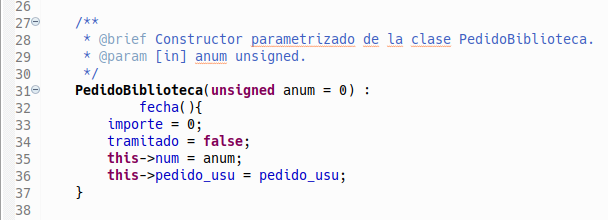
\includegraphics[scale=0.7]{img/captura53.png}
				\caption{Captura de pantalla del constructor parametrizado de la clase PedidoBiblioteca tras la corrección del error}
				\label{captura53}
			\end{figure}
		
			\paragraph{Nota:} Una segunda forma de corregir el error habría sido declarar el constructor como explícito, es decir, añadir \textit{explicit} a la declaración del constructor. Hemos descartado esta opción ya que en algunos casos esto podría ocasionar un comportamiento indeseado en la ejecución del programa en ciertas situaciones.

	\subsection{Error nº4: Parameter can be declared with const}
	
		\subsubsection{Origen/explicación del error detectado}
		
		\paragraph{}Este error tiene su origen en el constructor por copia de la clase \textit{PedidoBiblioteca}. A continuación, se presenta una captura de pantalla de dicho constructor.
		
		\begin{figure}[H]
			\centering
			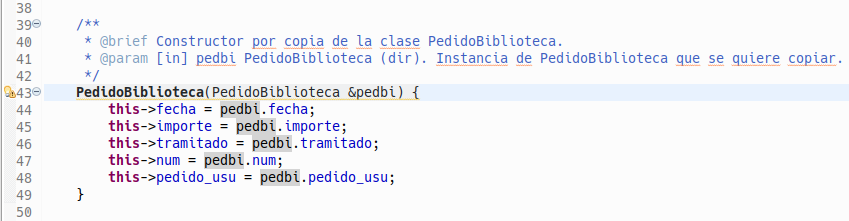
\includegraphics[scale=0.55]{img/captura54.png}
			\caption{Captura de pantalla del constructor por copia de la clase PedidoBiblioteca}
			\label{captura54}
		\end{figure}
	
		\paragraph{}Como se puede observar en la captura, cppcheck nos indica que el error se encuentra en la línea 43 del archivo. Nos recomienda que el parámetro \textit{pedbi} puede ser declarado como constante. Este parámetro es el la instancia del objeto del cuál se hace una copia
		
		\paragraph{}Es bastante común (y recomendable) que en los constructores por copia y en los operadores de asignación se pasen como constante los objetos de los cuales queremos copiar el valor de sus atributos. Esto se realiza para evitar que, bien por descuido o bien por error de programación, se modifiquen los valores de los atributos miembros de estos parámetros.
		
		\paragraph{}Es por este motivo que cppcheck nos avisa de que podemos hacer este parámetro constante.
		
		\paragraph{}Este error también es detectado para el parámetro \textit{pedbi}, en la línea 70 del archivo \textit{PedidoBiblioteca.h}; y para el parámetro \textit{pedido}, en la línea 49 del archivo \textit{PedidoUsuario.h}. A continuación, presentamos capturas de pantalla de las funciones en las que aparecen estos errores.
		
		\begin{figure}[H]
			\centering
			
\includegraphics[scale=0.38]{img/captura55.png}
			\caption{Detalle del mensaje de error de cppcheck}
			\label{captura55}
		\end{figure}
	
		\begin{figure}[H]
			\centering
			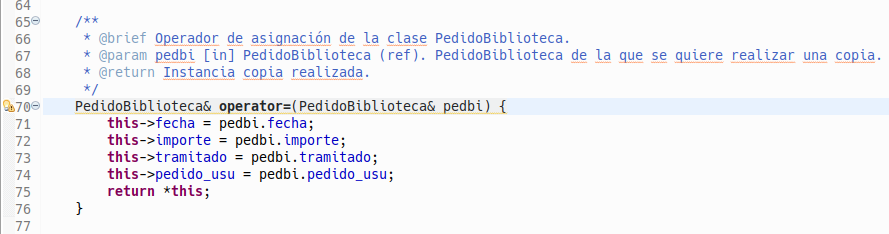
\includegraphics[scale=0.5]{img/captura57.png}
			\caption{Captura de pantalla del operador de asignación de la clase PedidoBiblioteca}
			\label{captura57}
		\end{figure}
	
		\begin{figure}[H]
			\centering
			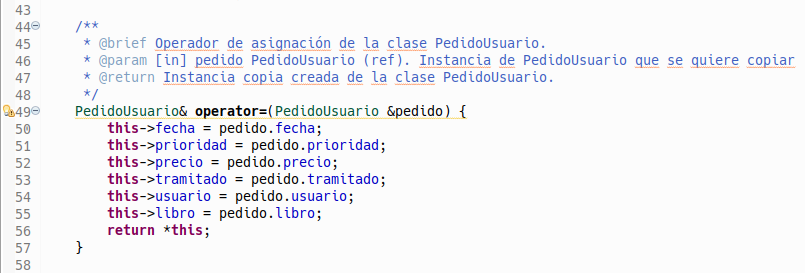
\includegraphics[scale=0.55]{img/captura58.png}
			\caption{Captura de pantalla del operador de asignación de la clase PedidoUsuario}
			\label{captura58}
		\end{figure}
	
		\subsubsection{Corrección realizada para solventar el error}
		
		\paragraph{}Para corregir este error tan solo deberemos hacer constante el parámetro \textit{pedbi}. Una vez hecho esto habrá desaparecido el aviso de cppcheck.
		
		\begin{figure}[H]
			\centering
			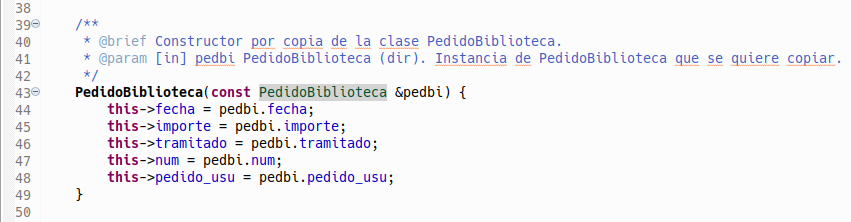
\includegraphics[scale=0.55]{img/captura56.png}
			\caption{Captura de pantalla del constructor por copia de la clase PedidoBiblioteca tras la corrección del error}
			\label{captura56}
		\end{figure}
	
		\begin{figure}[H]
			\centering
			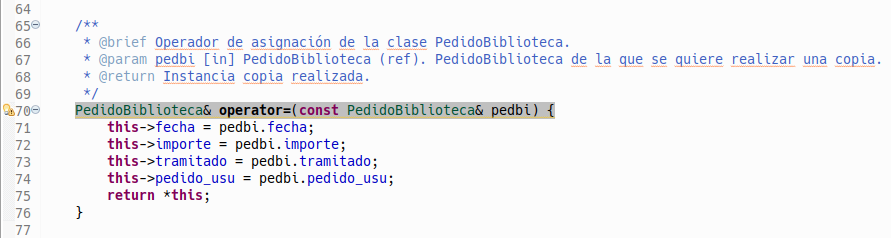
\includegraphics[scale=0.5]{img/captura59.png}
			\caption{Captura de pantalla del operador de asignación de la clase PedidoBiblioteca tras la resolución del error}
			\label{captura59}
		\end{figure}
	
		\paragraph{Nota:}El aviso que se muestra en la captura de pantalla se debe a otro origen; el error de este apartado ha sido solucionado.
		
		\begin{figure}[H]
			\centering
			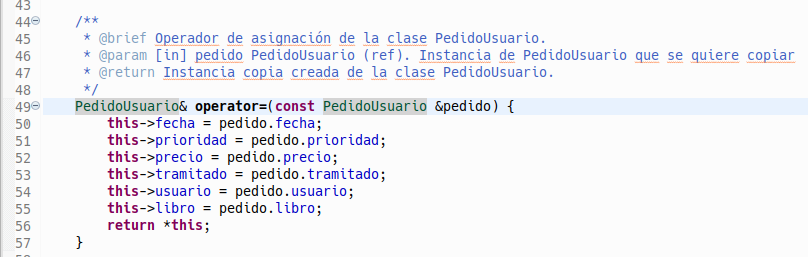
\includegraphics[scale=0.55]{img/captura60.png}
			\caption{Captura de pantalla del operador de asignación de la clase PedidoUsuario tras la resolución del error}
			\label{captura60}
		\end{figure}
		
		\paragraph{Nota:}En el caso de que en nuestro constructor ó función necesitáramos por algún motivo modificar el valor de alguno de los atributos miembro del parámetro y, aún así, nos saltara el aviso de cppcheck deberíamos hacer caso omiso ya que de este modo nos daría un error al compilar el código.
	
\newpage